\documentclass[11pt,a4paper]{article}

\usepackage{cmap}
\usepackage[utf8]{inputenc}
\usepackage[T1]{fontenc}
\usepackage{lmodern}
\usepackage[french]{babel}
\usepackage[a4paper,margin=2.35cm]{geometry}
\usepackage{graphicx}
\usepackage{booktabs}
\usepackage{array}
\usepackage{xcolor}
\usepackage{caption}
\usepackage{enumitem}
\usepackage{fancyhdr}
\usepackage{titlesec}
\usepackage[hidelinks]{hyperref}

\graphicspath{{figures/}}
\definecolor{nblue}{HTML}{1D3A6B}
\definecolor{acc}{HTML}{2563EB}
\definecolor{boxbg}{HTML}{EFF4FB}

\titleformat{\section}{\Large\bfseries\color{nblue}}{\thesection}{0.6em}{}
\titleformat{\subsection}{\large\bfseries\color{acc}}{\thesubsection}{0.6em}{}
\setlength{\parskip}{0.42em}
\setlength{\parindent}{0pt}
\setlist[itemize]{leftmargin=1.35em,itemsep=0.2em,topsep=0.2em}
\setlist[enumerate]{leftmargin=1.45em,itemsep=0.2em,topsep=0.2em}

\pagestyle{fancy}\fancyhf{}
\lhead{\small\color{nblue}Projet Machine Learning ASRS}
\rhead{\small\thepage}
\renewcommand{\headrulewidth}{0.4pt}
\captionsetup{font=small,labelfont={bf,color=nblue}}

% Exemple d'application : fondu dans le texte (pas d'encadré)
\newcommand{\exemple}[1]{\par\noindent #1}

\begin{document}

\begin{titlepage}
\centering
\vspace*{1.3cm}
{\small\color{acc}\textbf{PROJET MACHINE LEARNING}}\\[0.9cm]
{\color{nblue}\Huge\bfseries Analyse automatique des rapports\\[0.25cm] d'incidents NASA ASRS\par}
\vspace{0.5cm}
{\large Clustering thématique, classification des anomalies, signaux faibles\\ et tableau de bord d'aide à la décision\par}
\vspace{0.45cm}
{\itshape Rapport final académique}\par
\vspace{0.8cm}
\begin{tabular}{c}
{\Large\bfseries TIDJANI Mehdi}\\[0.25cm]
{\Large\bfseries FEUDJEU II LA GRACE}\\[0.25cm]
{\Large\bfseries OUEDRAOGO Martin}
\end{tabular}
\vfill
\begin{tabular}{r p{0.68\textwidth}}
\textbf{Données} & NASA ASRS -- 125\,763 rapports \\
\textbf{Source Kaggle} & \href{https://www.kaggle.com/datasets/mnhagemann21/nasa-asrs-full-dataset-20052025}{NASA ASRS Full Dataset 2005--2025} \\
\textbf{Période} & juin 2002 -- décembre 2025 \\
\textbf{Méthodes} & TF-IDF, embeddings, UMAP, HDBSCAN, LDA, SVM \\
\textbf{Livrables} & notebook, pipeline Python, dashboard Streamlit, dashboard React, rapport PDF \\
\textbf{Dépôt} & \url{https://github.com/devMehdi485/asrs-ml}
\end{tabular}
\vspace{0.8cm}
\end{titlepage}

\tableofcontents
\newpage

% ===================================================================
\section{Contexte}

La base NASA ASRS (\emph{Aviation Safety Reporting System}) regroupe des rapports
d'incidents aériens déclarés volontairement par les pilotes, contrôleurs et autres acteurs
opérationnels. Chaque rapport contient un récit en texte libre décrivant le contexte, le
déroulement de l'incident et les facteurs contributifs. Le projet exploite un export de
\textbf{125\,763 rapports} couvrant la période de juin 2002 à décembre 2025.

Le jeu de données utilisé est le dataset Kaggle \emph{NASA ASRS Full Dataset 2005--2025},
disponible sur
\href{https://www.kaggle.com/datasets/mnhagemann21/nasa-asrs-full-dataset-20052025}{Kaggle}.

% ===================================================================
\section{Problématique}

Le volume du corpus rend impossible toute lecture manuelle exhaustive, et l'information utile
est enfouie dans un texte non structuré et hétérogène. La problématique est donc :
\textbf{comment exploiter automatiquement les récits ASRS pour identifier les causes
récurrentes, classer les anomalies et détecter les risques émergents}, au service de la
sécurité aérienne ?

% ===================================================================
\section{Objectifs}

\begin{enumerate}
  \item identifier automatiquement les thèmes d'incidents récurrents ;
  \item classer les catégories d'anomalies à partir du texte ;
  \item détecter les signaux faibles et les risques émergents ;
  \item restituer les résultats dans un tableau de bord interactif.
\end{enumerate}

% ===================================================================
\section{Méthodologie}

La chaîne de traitement enchaîne cinq étapes. Chacune est décrite par son application
concrète au corpus ASRS et par le résultat obtenu, plutôt que par la théorie des algorithmes.

\subsection{Données}
Le pipeline charge l'export CSV, repère automatiquement les colonnes utiles (le format ASRS
comporte une double ligne d'en-tête) et fusionne les champs textuels (\emph{narrative}
Reporter 1 \& 2, synopsis) en un texte d'analyse par rapport. Les métadonnées (date, phase de
vol, type d'anomalie) sont conservées pour interpréter les résultats.
\exemple{Le corpus obtenu contient 125\,763 textes ; les champs textuels sont remplis à
100\,\% et le type d'anomalie à 99,7\,\%. Les phases de vol les plus représentées sont
\emph{Cruise} (20\,738 rapports), \emph{Parked} (15\,493), \emph{Initial Approach}
(12\,880), \emph{Taxi} (12\,294) et \emph{Climb} (11\,132).}

\subsection{Prétraitement}
Les textes sont nettoyés pour retirer le bruit propre au format ASRS : marqueurs
d'anonymisation (\texttt{ZZZ}, \texttt{XXX}), casse, ponctuation, mots très fréquents et
termes métier omniprésents (« aircraft », « flight »), puis lemmatisation des variantes.
\exemple{Sans ce nettoyage, les marqueurs \texttt{ZZZ} — présents dans presque tous les
rapports — domineraient les statistiques de mots. Après nettoyage, les termes extraits par
thème deviennent réellement discriminants : le thème des défaillances hydrauliques ressort
avec \texttt{hydraulic, pump, fluid} et non avec du vocabulaire générique.}

\subsection{Vectorisation}
Deux représentations sont produites : une matrice \textbf{TF-IDF} (mots et bigrammes) pour la
classification et l'extraction de mots-clés, et des \textbf{embeddings} de phrases
(\texttt{all-MiniLM-L6-v2}) qui encodent le sens global d'un récit pour le regroupement. Un
modèle Word2Vec entraîné sur le corpus a servi à contrôler la cohérence du vocabulaire.
\exemple{Le contrôle Word2Vec confirme que la sémantique aéronautique est bien captée :
\texttt{runway} est le plus proche de \texttt{rwy} (0,84) et de \texttt{taxiway} (0,65) ;
\texttt{weather} de \texttt{thunderstorm} (0,76). Les embeddings permettent de rapprocher
deux récits décrivant le même événement avec des mots différents — situation fréquente dans
des rapports rédigés librement — ce qui se traduit par un regroupement nettement plus
cohérent (silhouette de 0,590, \S\,5.1).}

\subsection{Clustering thématique}
Les embeddings sont réduits par UMAP, puis regroupés. Deux algorithmes ont été comparés sur
les mêmes données : K-Means et HDBSCAN. HDBSCAN a été retenu car il découvre lui-même le
nombre de groupes, gère des groupes de tailles très inégales et isole les rapports atypiques
(« bruit »), réutilisés ensuite pour la détection de signaux faibles.

Le regroupement produit une structure à trois niveaux :
\begin{center}\small
\fbox{\textbf{125\,763 rapports} (texte libre)}\\[3pt]
$\downarrow$\;\textit{regroupement automatique (HDBSCAN)}\\[3pt]
\fbox{\textbf{81 thèmes} fins — ex. « Pannes hydrauliques », « Train d'atterrissage », « Pression d'huile »}\\[3pt]
$\downarrow$\;\textit{regroupement manuel par familles}\\[3pt]
\fbox{\textbf{11 catégories} larges — ex. « Équipement \& systèmes », « Sol \& piste »}
\end{center}

\textbf{Nommage des thèmes (labellisation).} Les noms des 81 thèmes ont été déterminés de
façon semi-automatique. Pour chaque thème, les termes \emph{distinctifs} sont extraits
automatiquement par c-TF-IDF (une variante du TF-IDF appliquée au thème entier, qui retient
les mots fréquents dans ce thème mais rares ailleurs) ; ils sont croisés avec l'anomalie
dominante et trois récits représentatifs. À partir de ces éléments, un libellé métier lisible
est rédigé et consigné dans un fichier versionné. Le clustering et l'extraction des mots-clés
sont donc entièrement automatiques ; seule la mise en mots du nom relève d'une validation
humaine, et n'influence aucun résultat quantitatif.
\exemple{Le thème dont les termes c-TF-IDF sont \texttt{hydraulic · pump · fluid · system},
d'anomalie dominante \emph{Aircraft Equipment Problem Critical}, est nommé
« \textbf{Pannes hydrauliques} » et rattaché à la catégorie « Équipement \& systèmes ».}

\subsection{Classification}
Un modèle supervisé prédit la catégorie d'anomalie d'un rapport à partir de son texte complet
(et non de mots isolés). Deux modèles linéaires ont été entraînés sur la matrice TF-IDF —
régression logistique et SVM linéaire — restreints aux huit catégories d'anomalies les plus
fréquentes. Le choix de modèles linéaires permet de garder une décision auditable (les mots
déterminants sont lisibles), critère important en contexte de sécurité.
\exemple{Sur un rapport décrivant un franchissement de piste sans autorisation, le modèle
prédit la catégorie \emph{Conflit / incursion} avec une probabilité élevée, en s'appuyant sur
des termes comme \texttt{runway}, \texttt{hold short} et \texttt{clearance}.}

% ===================================================================
\section{Résultats}

\subsection{Cohérence des clusters}
La comparaison des deux algorithmes (tableau~\ref{tab:clust}) établit la supériorité
d'HDBSCAN : silhouette de 0,590 (contre 0,382) et indice de Davies-Bouldin de 0,575 (contre
0,945), traduisant des groupes plus compacts et mieux séparés. HDBSCAN forme 81 thèmes et
classe 32,5\,\% des rapports comme atypiques (« bruit »), réutilisés en \S\,5.4. La faible
concordance avec les catégories officielles (pureté de 0,165) n'est pas un défaut : elle
reflète la granularité plus fine des thèmes issus du texte par rapport à la nomenclature des
analystes.

\begin{figure}[h]\centering
  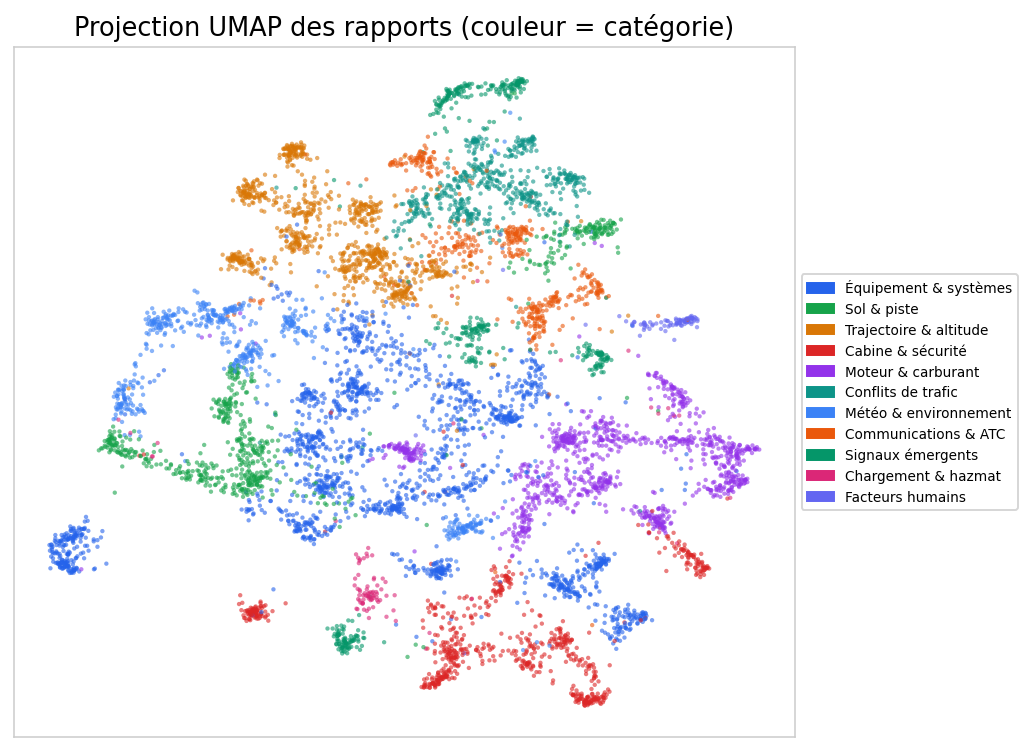
\includegraphics[width=0.82\textwidth]{scatter.png}
  \caption{Projection UMAP des rapports ASRS : chaque point représente un rapport et la
  couleur indique sa catégorie thématique.}\label{fig:umap}
\end{figure}

\begin{table}[h]\centering\small
\caption{Indices internes de qualité du regroupement.}\label{tab:clust}
\begin{tabular}{lrrrrr}
\toprule
\textbf{Algorithme} & \textbf{Groupes} & \textbf{Silhouette} & \textbf{Davies-Bouldin} & \textbf{Bruit} & \textbf{Pureté} \\
\midrule
K-Means & 15 & 0,382 & 0,945 & 0\,\% & 0,133 \\
HDBSCAN & 81 & 0,590 & 0,575 & 32\,\% & 0,165 \\
\bottomrule
\end{tabular}
\end{table}

\subsection{Interprétation des thèmes}
Les 81 thèmes se répartissent en 11 catégories (figure~\ref{fig:cat}). La catégorie
\textbf{Équipement \& systèmes} domine avec \textbf{43,8\,\%} des rapports, devant
\textbf{Sol \& piste} (13,3\,\%) et \textbf{Trajectoire \& altitude} (7,8\,\%). Cette
prédominance s'interprète comme une forte propension des équipages à signaler les
dysfonctionnements techniques.

\begin{figure}[h]\centering
  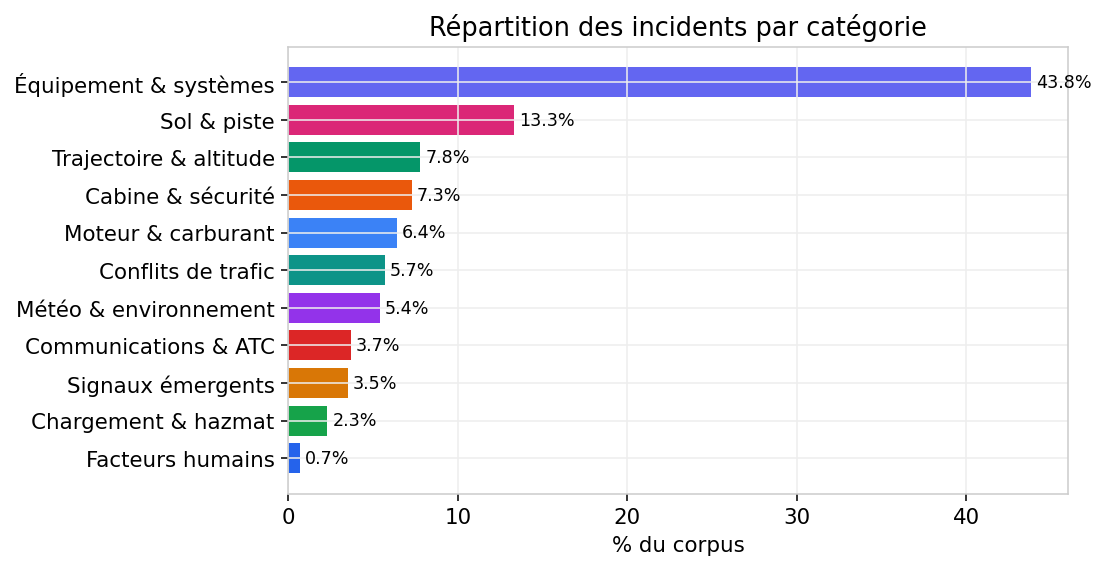
\includegraphics[width=0.78\textwidth]{categories.png}
  \caption{Répartition des rapports par catégorie (81 thèmes regroupés en 11 familles).}\label{fig:cat}
\end{figure}

Concrètement, les thèmes les plus volumineux (figure~\ref{fig:top}) sont : pannes avioniques
et systèmes (22\,258 rapports), incursions et erreurs au sol (8\,458), fumées et odeurs en
cabine (3\,392), conflits de trafic en circuit d'aérodrome (2\,656), turbulence de sillage
(2\,459), maintenance et inspections (2\,108), chargement et marchandises dangereuses
(1\,959), proximité du terrain à l'approche (1\,907), coordination ATC (1\,858) et problèmes
de train d'atterrissage (1\,804).

\begin{figure}[h]\centering
  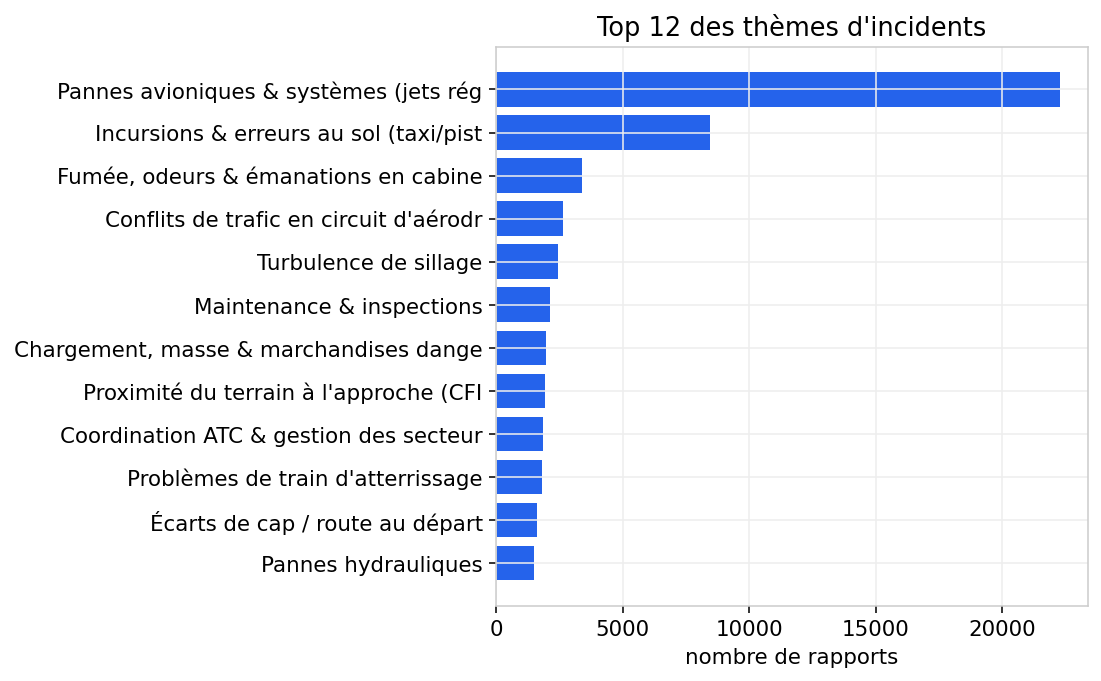
\includegraphics[width=0.78\textwidth]{top_themes.png}
  \caption{Douze thèmes les plus volumineux.}\label{fig:top}
\end{figure}

Pour interpréter rapidement un thème, le tableau de bord en affiche le \textbf{nuage de
mots} : les termes les plus distinctifs y sont dimensionnés selon leur importance, ce qui
permet d'identifier le contenu d'un thème d'un coup d'œil sans lire les rapports
(figure~\ref{fig:wc}).

\begin{figure}[h]\centering
  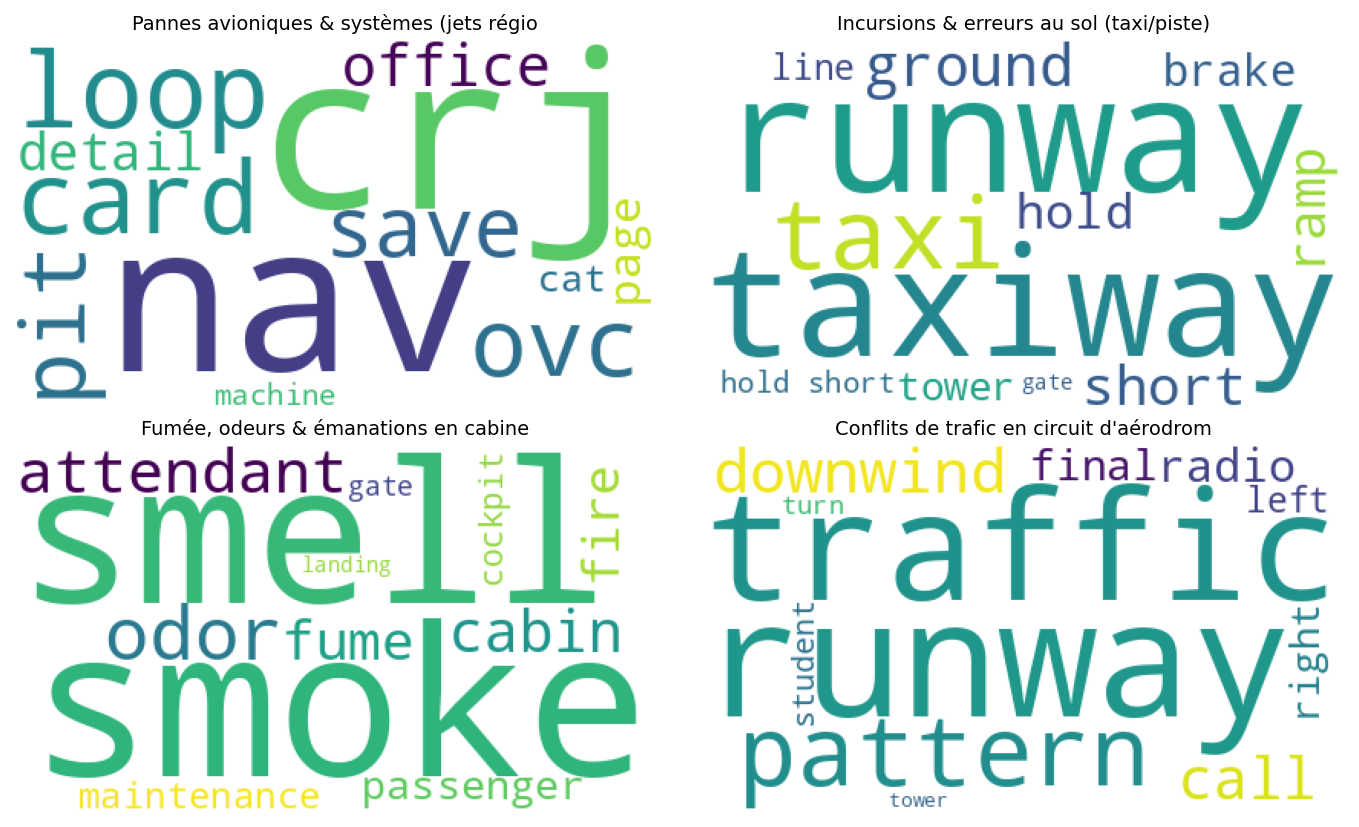
\includegraphics[width=0.9\textwidth]{wordclouds.png}
  \caption{Nuages de mots des quatre principaux thèmes : les termes distinctifs (taille
  proportionnelle à l'importance) résument le contenu de chaque thème.}\label{fig:wc}
\end{figure}

\subsection{Performance de la classification}
Le SVM linéaire atteint un \textbf{F1 pondéré de 0,615} (tableau~\ref{tab:clf}). L'écart avec
le F1 macro (0,517) traduit l'effet du déséquilibre des classes : les catégories au
vocabulaire spécifique sont bien reconnues — \emph{ATC Issue} (F1 = 0,76), \emph{Conflict
NMAC} (0,69), \emph{Aircraft Equipment Problem Critical} (0,67) — tandis que les classes
rares abaissent la moyenne.

\begin{table}[h]\centering\small
\caption{Classification de la catégorie d'anomalie (8 classes, entrées TF-IDF).}\label{tab:clf}
\begin{tabular}{lrr}
\toprule
\textbf{Modèle} & \textbf{F1 macro} & \textbf{F1 pondéré} \\
\midrule
Régression logistique & 0,518 & 0,606 \\
SVM linéaire & 0,517 & 0,615 \\
\bottomrule
\end{tabular}
\end{table}

\subsection{Signaux faibles détectés}
La détection d'anomalies (Isolation Forest sur les représentations, complétée par le bruit
HDBSCAN) isole les rapports les plus atypiques. Leur examen fait ressortir des thématiques
rares mais à fort enjeu, quasi absentes en début de période : \textbf{rencontres avec des
drones}, \textbf{brouillage du signal GPS} et \textbf{batteries au lithium}. Un rapport
représentatif illustre la catégorie « drones » :

\begin{quote}\small\itshape\color{nblue}
\guillemotleft~Approach control advised there was unauthorized drone use in the area\ldots I
observed a drone pass just left of the aircraft, approximately 20 feet from our left
wing.~\guillemotright
\end{quote}

\noindent L'évolution temporelle (figure~\ref{fig:heat}) confirme par ailleurs la
\textbf{progression récente} de trois thèmes : incursions au sol, fumées en cabine et
marchandises dangereuses.

\begin{figure}[h]\centering
  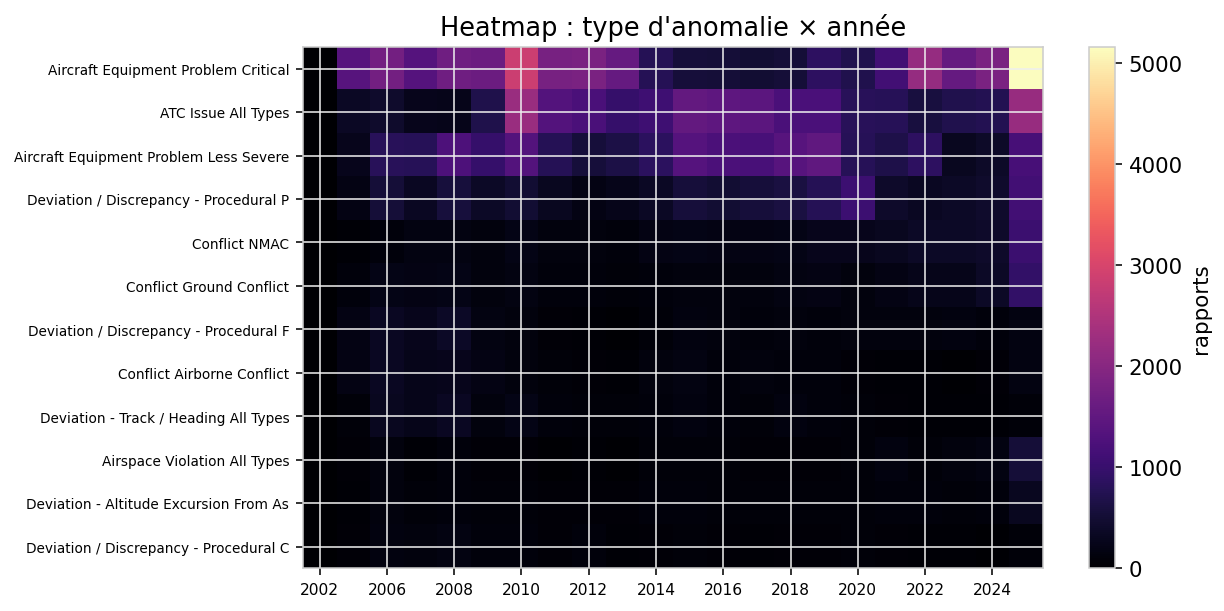
\includegraphics[width=0.84\textwidth]{heatmap.png}
  \caption{Répartition des principales anomalies par année (intensité relative à chaque
  type) : une ligne qui se réchauffe vers la droite indique un type d'incident en
  progression.}\label{fig:heat}
\end{figure}

% ===================================================================
\section{Tableau de bord}

Les résultats sont restitués dans deux tableaux de bord interactifs : une version
\textbf{Streamlit} (Python) et une application web \textbf{React} (« AeroInsight AI »).

La version Streamlit a été simplifiée pour l'usage de présentation. Elle contient uniquement
deux vues :
\begin{itemize}
  \item le \textbf{nuage de mots par cluster}, qui permet de comprendre rapidement le contenu
  d'un thème ;
  \item la \textbf{carte temporelle des incidents}, qui montre l'évolution des volumes et des
  anomalies dans le temps.
\end{itemize}

La version React sert de tableau de bord complet. Elle permet d'explorer les catégories, les
thèmes, les tendances temporelles, les signaux faibles et la prédiction d'anomalies.
L'objectif est de rendre les résultats consultables par un lecteur non spécialiste du code.

% ===================================================================
\section{README -- lancement du dashboard}

Pour lancer le dashboard React en local :

\begin{verbatim}
cd frontend
npm install
npm run dev
\end{verbatim}

L'application est ensuite disponible dans le navigateur à l'adresse indiquée par Vite
(généralement \url{http://localhost:5173}).

Pour lancer la version Streamlit :

\begin{verbatim}
streamlit run dashboard/app.py
\end{verbatim}

% ===================================================================
\section{Implications et recommandations}

Les résultats se traduisent en pistes concrètes pour la sécurité aérienne :
\begin{itemize}
  \item \textbf{Équipement (43,8\,\%) et maintenance.} Le volume des signalements techniques
  plaide pour une \textbf{maintenance prédictive} exploitant ces remontées.
  \item \textbf{Incursions au sol (en hausse).} Cohérentes avec la densification du trafic,
  elles justifient un renforcement des procédures de roulage, du marquage des aires de
  manœuvre et de la vigilance ATC au sol.
  \item \textbf{Fumées et odeurs en cabine (en hausse).} Appellent une surveillance accrue de
  la qualité de l'air et des circuits de prélèvement.
  \item \textbf{Marchandises dangereuses (en hausse).} Justifient un contrôle documentaire
  renforcé du fret.
  \item \textbf{Risques émergents (drones, GPS, lithium).} Recommandent une veille dédiée et
  l'évaluation de moyens de détection et de contre-mesures.
\end{itemize}

% ===================================================================
\section{Conclusion}

Le projet livre une chaîne complète exploitant automatiquement 125\,763 rapports d'incidents
en texte libre. Le regroupement non supervisé identifie 81 thèmes interprétables (silhouette
de 0,590), agrégés en 11 catégories ; la classification supervisée atteint un F1 pondéré de
0,615 ; la détection d'anomalies fait remonter des risques émergents. L'ensemble transforme
une masse de récits dispersés en information structurée et exploitable, restituée dans un
tableau de bord, et fournit des recommandations concrètes pour la sécurité aérienne.

\vfill
\noindent\footnotesize\textit{Sources des données : NASA Aviation Safety Reporting System
(\url{https://asrs.arc.nasa.gov/}) et dataset Kaggle
\url{https://www.kaggle.com/datasets/mnhagemann21/nasa-asrs-full-dataset-20052025}. Code,
dashboards et reproductibilité : \url{https://github.com/devMehdi485/asrs-ml}.}

\end{document}
